\documentclass{standalone}
\usepackage[dvipsnames]{xcolor}
\usepackage{tikz}
\usepackage{graphicx}
\usepackage{pgf}

\usetikzlibrary{patterns, shapes}

\begin{document}

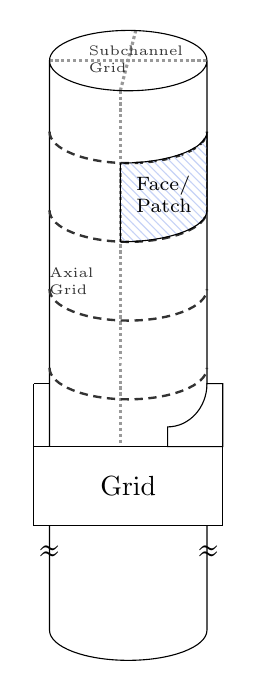
\begin{tikzpicture}
% define variables
\pgfmathparse{0.7}\let\r=\pgfmathresult
\linespread{1}% <--- locally defined vertical line spacing in nodes

% subchannel markings
\draw[densely dotted, black!40, line width=0.04cm] (-1, 3.9) -- (1.0, 3.9);
\draw[densely dotted, black!40, line width=0.04cm] (-0.1, 3.52) -- (0.1, 4.3);
\draw[densely dotted, black!40, line width=0.04cm] (-0.1, 3.52) -- (-0.1, -1.0);
\node[text width=1.0cm, black!80, font=\tiny] at (0, 3.92) {Subchannel Grid};

% draw cylender
\node (A) [cylinder, shape border rotate=90, draw,minimum height=8cm,minimum width=2cm] {\color{white} Pin};

% draw ctf axial grid
\foreach \y in {0, 1, 2, 3}{
\draw[densely dashed, black!80, line width=0.03cm] (-1,\y) arc (180:360:1.0cm and 0.4cm) ;
}
\node[text width=1.0cm, black!80, font=\tiny] at (-0.5, 1.1) {Axial Grid};

% draw shaded region
\draw[pattern=north west lines,pattern color=RoyalBlue!30] (-0.1, 1.6) -- (-0.1, 2.6) arc (270:360:1.1cm and 0.4cm) -- (1.0, 2.0) arc (360:270:1.1cm and 0.4cm) ;
\node[text width=1.0cm, font=\scriptsize] at (0.6, 2.2) {Face/ Patch};
%\draw (-0.1, 2.6) arc (270:360:1.1cm and 0.4cm);
%\draw (-0.1, 1.6) arc (270:360:1.1cm and 0.4cm);
%\draw (-0.1, 1.6) -- (-0.1, 2.6);
%\draw (1.0,  3.0) -- (1.0, 2.0);

% draw grids
\draw[fill=white] (-1.2,-2.0) rectangle (1.2,-1.0) node[pos=0.5] {Grid};
\draw[-] (-1.2,-1.0) -- (-1.2, -0.2);
\draw[-] (-1.2, -0.2) -- (-1.0, -0.2);
\draw[fill=white] (0.5, -1.0) -- (0.5, -0.75) arc (270:360:0.5cm and 0.55cm) -- (1.2, -0.2) -- (1.2, -1.0) -- cycle;


% draw inf marks
\node[text width=1cm, font=\huge] at (-0.66,-2.5) { \~~ };
\node[text width=1cm, font=\huge] at (-0.66,-2.58) { \~~ };
%
\node[text width=0.3cm, font=\huge] at (1.0,-2.5) { \~~ };
\node[text width=0.3cm, font=\huge] at (1.0,-2.58) { \~~ };

\end{tikzpicture}



\end{document}
